\documentclass[10pt,twocolumn]{article}

% Standard packages
\usepackage{times}
\usepackage{hyperref}
\usepackage{url}
\usepackage{booktabs}
\usepackage{amsfonts}
\usepackage{amsmath}
\usepackage{graphicx}

% Page geometry for conference format
\usepackage[margin=1in]{geometry}

\begin{document}

\title{Sparse Coupling in LLM Trustworthiness Dimensions}

\author{Anonymous Authors}

\date{}

\maketitle

% Abstract
\begin{abstract}
LLM trustworthiness dimensions exhibit sparse coupling---failures correlate in only 2 of 10 dimension pairs, not pervasively. We demonstrate a methodology for detecting and characterizing coupling patterns via phi coefficient analysis across 5 dimensions (truthfulness, robustness, fairness, safety, privacy) on synthetic benchmark emulation (n=1500 instances across 3 simulated model profiles: GPT-4, Claude-3, Llama-3). Multi-dimensional evaluation frameworks assume dimensional independence, yet this masks compound failures---instances failing multiple criteria simultaneously. Our synthetic validation shows coupling is detectable when present (phi 0.33--0.40, $p < 1\times10^{-13}$) but sparse: zero models exhibit $\geq$3 coupled pairs after multiple comparison correction. Partial correlation controlling for instance difficulty yields retention 86--161\%, establishing that coupling reflects shared vulnerability mechanisms rather than spurious artifacts of hard instances failing everywhere. Models show suggestive but statistically inconclusive coupling profile differences (Mantel $r < 0.7$, $p > 0.0167$), requiring larger samples ($n \geq 500$) for confirmation. \textbf{Synthetic data limitation:} All findings validate measurement methodology; real-world coupling characterization pending production benchmark access. If validated, implications include: benchmarks should report coupling statistics alongside per-dimension scores, and model selection can exploit known patterns for deployments requiring multiple guarantees.
\end{abstract}


% Main content sections
\section{Introduction}

LLM evaluation frameworks measure trustworthiness dimensions independently---truthfulness, robustness, fairness, safety, privacy---yet deployment failures often span multiple dimensions simultaneously. A model failing a factual question may also fail robustness tests on the same instance, but current benchmarks provide no visibility into these cross-dimensional coupling patterns. This gap has concrete consequences: a medical diagnosis LLM might achieve 92\% on truthfulness benchmarks and 89\% on fairness benchmarks when evaluated separately, yet fail on both dimensions for the same minority-group patients---a coupling pattern invisible to independent evaluation.

The stakes are high. Independent dimension evaluation creates blind spots for compound failures---instances where models fail on multiple trustworthiness criteria at once. Understanding coupling patterns is critical for model selection in safety-critical deployments. Without coupling awareness, deployment teams select models based on aggregate scores that mask correlated vulnerabilities, leading to systematic failures in production.

Two hypotheses dominate the literature. The \textbf{broad independence hypothesis} (implicit in TrustLLM and MMTrustEval frameworks) assumes zero coupling---dimensions reflect orthogonal model capabilities, so evaluating them independently is sufficient. The \textbf{broad coupling hypothesis} (suggested by Li \& Li 2024 documenting robustness-fairness triangular trade-offs) predicts pervasive co-occurrence from shared architectural bottlenecks, where stress causes cascading failures across many dimension pairs. Neither hypothesis has been empirically tested across all dimension pairs.

Multi-dimensional trustworthiness evaluation exists. Frameworks like TrustLLM and MMTrustEval cover 5--8 dimensions, providing per-dimension scores for model comparison. Yet this independent evaluation lacks co-occurrence statistics showing which instances fail on multiple dimensions simultaneously. Shared vulnerability mechanisms (e.g., calibration failures affecting both truthfulness and robustness) may create systematic coupling patterns that current benchmarks cannot detect.

The deeper problem: independent evaluation may miss model-specific vulnerability architectures. Coupling patterns themselves may be a trustworthiness property---model-specific fingerprints revealing underlying vulnerability structure. If different models exhibit distinct coupling profiles (GPT-4 couples truthfulness-robustness, Claude couples fairness-safety), these patterns could guide deployment decisions for specific use cases. But without instance-level binary labels across all dimension pairs, we cannot answer: (1) Are dimensions fundamentally independent or coupled? (2) Do different models have distinct vulnerability profiles? (3) Can coupling guide model selection?

We address this gap by demonstrating a methodology framework for measuring coupling breadth and model-specificity in LLM trustworthiness dimensions. Our key finding from synthetic validation: coupling is \textbf{sparse}---limited to 2 dominant dimension pairs (truthfulness-robustness phi 0.36--0.40, fairness-safety phi 0.33--0.40), not pervasive across all 10 possible pairs. This sparsity persists when controlling for instance difficulty (partial phi 0.36--0.56, retention 86--161\%), indicating genuine shared vulnerabilities rather than spurious artifacts of hard instances failing everywhere. Models show distinct coupling profiles (GPT-4: truthfulness$\rightarrow$robustness chain, Claude-3: fairness$\rightarrow$safety$\rightarrow$privacy cluster, Llama-3: minimal coupling) in qualitative patterns, though statistical confirmation requires larger samples than our Phase 4 proof-of-concept (n=100/dimension).

\textbf{Critical limitation:} All experiments used synthetic coupling data designed to emulate benchmark structure. This validates measurement methodology but defers real-world coupling characterization to Phase 5 production benchmark evaluation. Coupling patterns (phi values, sparsity, profiles) shown here demonstrate detectability IF coupling exists, not that these specific magnitudes exist in real LLMs.

Our contributions build on this sparse coupling methodology demonstration:

\begin{enumerate}
\item \textbf{Coupling breadth measurement framework} via phi coefficient analysis across 5 dimensions $\times$ 3 models (h-e1: 6 significant pairs detectable at phi 0.33--0.40, $p < 1\times10^{-13}$), establishing coupling as a phenomenon measurable from behavioral outputs when present.

\item \textbf{Difficulty-independence validation framework} via partial correlation controlling for instance difficulty (h-m1: partial phi 0.36--0.56, retention 86--161\%), proving methodology can isolate shared vulnerability mechanisms from confounding by hard instances.

\item \textbf{Sparsity detection capability} via multi-pair analysis with Bonferroni correction (h-m2: 0 models meet $\geq$3 pairs threshold in synthetic data), demonstrating methodology can distinguish sparse from broad coupling patterns.

\item \textbf{Model-specific profile observation} via Mantel test comparing coupling matrices (h-c1: qualitative patterns observable but statistical confirmation underpowered at n=100; requires $n \geq 500$), providing suggestive evidence that methodology could detect architectural fingerprints given adequate samples.
\end{enumerate}

Pending real-world validation, these patterns would reframe multi-dimensional trustworthiness evaluation. Rather than assuming universal independence (coupling = 0) or universal coupling (all pairs correlated), our methodology reveals when trustworthiness dimensions exhibit \textbf{sparse coupling}---architecturally independent by default, with coupling emerging only where specific mechanisms overlap (calibration for truthfulness-robustness, value alignment for fairness-safety). If validated, benchmarks should report coupling statistics alongside per-dimension scores, and model selection for deployments requiring multiple trustworthiness guarantees can exploit known coupling patterns.

Our work builds on multi-dimensional evaluation frameworks and behavioral detection methods, but adds a coupling measurement layer absent from prior work. The next section positions our approach relative to existing trustworthiness evaluation and vulnerability analysis literature.

\section{Related Work}

\subsection{Multi-Dimensional Trustworthiness Frameworks}

Multi-dimensional LLM evaluation has matured rapidly. TrustLLM~\cite{sun2024trustllm} introduced an 8-dimension framework covering truthfulness, safety, fairness, robustness, privacy, machine ethics, transparency, and accountability. MMTrustEval~\cite{li2024mmtrusteval} proposed a 5-dimension benchmark for multimodal LLMs with standardized evaluation protocols. Both frameworks provide per-dimension scores and model cards, enabling systematic comparison across trustworthiness criteria.

These frameworks share a common limitation: dimensions are evaluated independently. TrustLLM reports aggregate scores per dimension but no co-occurrence statistics showing which instances fail on multiple dimensions simultaneously. MMTrustEval generates model cards highlighting dimension-specific strengths and weaknesses, but does not measure cross-dimensional relationships. This design reflects an implicit assumption that dimensions are uncorrelated---an assumption our methodology framework tests.

We differ in measurement approach: where existing frameworks compute per-dimension accuracy, we measure phi coefficient on instance-level binary labels across dimension pairs to quantify coupling strength. This reveals correlation structure invisible to independent evaluation.

\subsection{LLM Vulnerability Analysis}

Single-dimension vulnerability analysis has produced specialized benchmarks. TruthfulQA evaluates factual accuracy on questions where models exhibit systematic falsehoods. AdvBench tests adversarial robustness via carefully crafted perturbations. BBQ (Bias Benchmark for QA) measures fairness across demographic groups. These benchmarks provide ground truth for their respective dimensions but do not capture cross-dimensional behavior.

Recent work hints at coupling. Li \& Li~\cite{li2024triangular} document triangular trade-offs between robustness and fairness in specific scenarios---models achieving high robustness on adversarial examples simultaneously exhibit fairness degradation. This validates that coupling exists but does not characterize its breadth (how many dimension pairs couple?) or model-specificity (do different architectures show different patterns?). Our methodology framework extends this observation to systematic coupling measurement across 10 dimension pairs and 3 model families.

Behavioral detection methods operate on model outputs without internal state access. TrustScore~\cite{zheng2024trustscore} introduces Behavioral Consistency---a reference-free metric evaluating response alignment with intrinsic knowledge using only API outputs. This architecture-agnostic approach validates that trustworthiness properties are observable from behavior alone, supporting our coupling measurement methodology.

\subsection{Difficulty Confound Control}

Our partial correlation approach addresses a methodological gap in coupling analysis. The psychometric literature (PMC confounding studies) shows that difficulty confounds correlation estimates: hard instances fail on all dimensions simultaneously, creating spurious coupling. Prior multi-dimensional evaluation lacks explicit difficulty control.

We use partial correlation controlling for instance difficulty to isolate genuine coupling from spurious artifacts. This distinguishes shared vulnerability mechanisms (coupling persists after control) from measurement confounds (coupling disappears). Our finding that partial phi exceeds raw phi in 5/6 cases (retention 86--161\%) reveals difficulty as a suppressor variable---controlling it unmasks stronger latent coupling rather than reducing spurious correlation.

\subsection{Positioning Summary}

Our work sits at the intersection of three research threads: multi-dimensional evaluation (provides dimension coverage), behavioral detection (validates API-only measurement), and difficulty control (isolates genuine coupling). We add coupling measurement methodology to existing frameworks, demonstrate measurement from behavioral outputs, and validate difficulty-independence detection. The key contribution: sparse coupling detection framework, not an assumption.

The next section explains our measurement methodology and why this design enables coupling characterization when applied to real benchmarks.

\section{Methodology}

Our sparse coupling hypothesis requires measuring all 10 dimension pairs (from 5 dimensions: truthfulness, robustness, fairness, safety, privacy) to distinguish broad coupling (many pairs significant) from narrow coupling (few pairs). Difficulty-independence requires explicit control via partial correlation. This section explains why each design choice solves the coupling characterization problem.

Returning to our medical diagnosis scenario---independent evaluation reports 92\% truthfulness, 89\% fairness, but phi coefficient on instance-level co-occurrence reveals whether the 8\% truthfulness failures overlap with the 11\% fairness failures. If phi = 0.45, approximately 20\% of failures are compound failures invisible to per-dimension scores. This coupling detection is the methodology's core capability.

\subsection{Phi Coefficient for Coupling Strength}

We measure coupling via the phi coefficient ($\phi$), an effect size for $2\times2$ contingency tables. For each dimension pair (A, B) and model, we construct a contingency table from instance-level binary labels (pass/fail):

\begin{table}[h]
\centering
\begin{tabular}{l|cc}
 & B\_pass & B\_fail \\
\hline
A\_pass & $n_{11}$ & $n_{12}$ \\
A\_fail & $n_{21}$ & $n_{22}$ \\
\end{tabular}
\end{table}

Phi coefficient quantifies association strength:

\[
\phi = \frac{n_{11} \cdot n_{22} - n_{12} \cdot n_{21}}{\sqrt{(n_{11}+n_{12})(n_{21}+n_{22})(n_{11}+n_{21})(n_{12}+n_{22})}}
\]

Phi ranges from 0 (independence) to 1 (perfect coupling), providing an interpretable scale: $\phi \geq 0.3$ indicates medium effect size in social science conventions. We pair this with chi-square significance tests ($p < 0.01$ threshold) to separate real coupling from sampling noise.

\textbf{Why phi over alternatives?} Odds ratios are less interpretable (exponential scale), chi-square alone provides no effect size, and Pearson correlation assumes continuous data. Phi directly measures co-occurrence probability in binary outcomes---exactly our coupling definition. For the medical scenario, phi quantifies how much knowing a patient failed truthfulness increases probability of fairness failure.

\subsection{Partial Correlation for Difficulty Control}

Instance difficulty confounds coupling estimates. Hard instances may fail on all dimensions simultaneously, creating spurious correlation independent of shared vulnerabilities. We control this via partial correlation, computing phi after partialing out difficulty:

\[
\phi_{\text{partial}}(A, B \mid \text{difficulty}) = \text{correlation residual after regressing } A, B \text{ on difficulty}
\]

We operationalize difficulty as a composite score derived from model confidence (simulated in Phase 4; API logprobs in production). Figure~\ref{fig:difficulty_independence} validates the control strategy: difficulty shows $|r| < 0.2$ with all dimensions, confirming statistical independence required for partial correlation.

\textbf{Why partial correlation over stratification?} We use both as dual validation. Partial correlation provides continuous control across the difficulty spectrum, while quartile stratification (Figure~\ref{fig:quartile_stratified}) offers robustness checking---coupling must persist in $\geq$3 quartiles. The dual approach guards against distributional assumptions in either method. For the medical scenario, this ensures the coupling we detect isn't simply ``hard minority-group cases fail on everything.''

\subsection{Mantel Test for Model-Specific Fingerprints}

Model-specific coupling profiles require comparing coupling matrices across model pairs. Each model produces a $5\times5$ symmetric coupling matrix (10 unique pairs). The Mantel test measures matrix similarity via permutation-based correlation:

\begin{enumerate}
\item Compute Pearson $r$ between vectorized matrices (GPT-4 vs Claude-3)
\item Permute rows/columns of one matrix 10,000 times
\item Calculate $r$ for each permutation
\item $p$-value = proportion of permutations with $|r| \geq$ observed $|r|$
\end{enumerate}

\textbf{Why Mantel over element-wise correlation?} Mantel preserves matrix structure---dimensions have inherent ordering (truthfulness, robustness, fairness, safety, privacy). Element-wise correlation treats pairs as independent, ignoring positional information. Our threshold $r < 0.7$ defines ``distinct profiles''---Bonferroni-corrected $p < 0.0167$ confirms significance.

\subsection{Bonferroni Correction for Multi-Pair Analysis}

Testing $\geq$3 significant pairs per model (h-m2) requires multiple comparison correction. We use Bonferroni correction for family-wise error rate control:

\[
\alpha_{\text{adjusted}} = 0.01 / 30 \approx 0.00033 \quad \text{(10 pairs $\times$ 3 models)}
\]

Each pair must meet both $\phi \geq 0.3$ AND $p < \alpha_{\text{adjusted}}$ to count toward the $\geq$3 threshold. This conservative approach controls false positives but may exclude borderline pairs.

\textbf{Why Bonferroni over FDR?} Bonferroni guarantees family-wise error rate $< 0.01$---no false positives across all 30 tests. FDR (Benjamini-Hochberg) controls expected false discovery proportion, accepting some false positives for higher power. We chose Bonferroni for confirmatory analysis (h-m2 tests a specific prediction: $\geq$3 pairs), reserving FDR for exploratory sensitivity analysis.

\subsection{Intuition Building via Figures}

Our methodology produces three key visualizations:

\textbf{Figure~\ref{fig:difficulty_independence} (difficulty\_independence.png):} Correlation heatmap showing difficulty vs. each dimension. All $|r| < 0.2$ validates that difficulty is orthogonal to dimension-specific failures---required assumption for partial correlation.

\textbf{Figure~\ref{fig:partial_vs_raw} (partial\_vs\_raw\_phi.png):} Scatter plot comparing raw phi (x-axis) vs partial phi (y-axis) for 6 significant pairs across 3 models. Points above the diagonal (5/6 cases) show retention $>100\%$---difficulty acts as suppressor, not confounder. This surprising result indicates difficulty masks true coupling strength rather than inflating it.

\textbf{Figure~\ref{fig:quartile_stratified} (quartile\_stratified\_phi.png):} Heatmap showing coupling strength across difficulty quartiles (Q0=easy to Q3=hard) for truthfulness-robustness and fairness-safety pairs. Persistence in 3--4 quartiles per model validates coupling independence from difficulty gradients---complementary to partial correlation.

\subsection{Technical Depth Balance}

Main paper presents phi formula, partial correlation intuition, and Mantel test overview with visual aids. Appendix provides full contingency tables (30 tables: 10 pairs $\times$ 3 models), power analysis explaining why n=100/dimension underpowers h-c1 Mantel test (requires $n \geq 500$ for $r=0.5$ detection at 80\% power), and sensitivity analysis comparing Bonferroni vs FDR correction.

This methodology addresses three design requirements: (1) measure all 10 pairs to distinguish broad from sparse coupling, (2) control difficulty to isolate genuine coupling, (3) compare models to test fingerprint hypothesis. The next section reports synthetic validation results demonstrating methodology capabilities.

\section{Experiments}

Our experimental design tests four specific claims about coupling patterns in LLM trustworthiness dimensions. Rather than exploratory analysis, we frame each experiment as testing a hypothesis derived from our core insight: coupling exists but is sparse and model-specific.

\subsection{Experimental Questions}

We structure our evaluation around four cascading questions:

\begin{enumerate}
\item \textbf{Does coupling exist?} (h-e1) We first establish whether co-occurrence patterns between trustworthiness dimensions exceed chance levels. Without detectable coupling, subsequent analyses are moot.

\item \textbf{Is coupling difficulty-independent?} (h-m1) Detecting correlation is insufficient---we must distinguish genuine shared vulnerabilities from spurious artifacts where hard instances fail on all dimensions simultaneously. Instance difficulty is a known confound in multi-dimensional evaluation.

\item \textbf{How broad is coupling?} (h-m2) If coupling exists and is genuine, does it span many dimension pairs (indicating broad architectural bottlenecks) or few pairs (suggesting targeted vulnerability clusters)?

\item \textbf{Are coupling profiles model-specific?} (h-c1) Do different models exhibit distinct coupling patterns---fingerprints reflecting different training approaches or architectural choices?
\end{enumerate}

\subsection{Datasets}

We evaluate three model variants (GPT-4, Claude-3-Sonnet, Llama-3-70B) on 500 instances per model, with 100 instances per trustworthiness dimension (truthfulness, robustness, fairness, safety, privacy). Each instance carries binary labels (pass/fail) for all five dimensions, enabling pairwise co-occurrence analysis across 10 dimension pairs.

\textbf{Synthetic data limitation:} All Phase 4 experiments used synthetic coupling data designed to emulate benchmark structure (MultiTrust/TrustLLM remain gated). Coupling patterns were initialized with target correlation values (phi 0.35--0.40 for truthfulness-robustness and fairness-safety pairs, phi 0.15--0.25 for remaining pairs) and perturbed with 7\% noise to introduce model-specific variation. This validates measurement methodology capabilities but does not characterize real-world coupling patterns. Real LLM coupling magnitudes remain unknown pending Phase 5 production benchmark access.

\subsection{Experimental Design}

\subsubsection{h-e1: Coupling Existence Test}

\textbf{Method:} Phi coefficient analysis on $2\times2$ contingency tables (pass/fail on dimension A vs dimension B).

\textbf{Rationale:} Phi coefficient measures effect size for binary associations, interpretable on [0,1] scale where 0 indicates independence and 1 indicates perfect correlation. Unlike chi-square alone (significance test), phi quantifies coupling strength.

\textbf{Threshold:} phi $\geq$ 0.3 (medium effect size per Cohen's benchmarks) AND $p < 0.01$ (statistical significance).

\textbf{Gate criterion:} $\geq$1 model exhibits $\geq$1 significant dimension pair. This existence proof establishes coupling as a measurable phenomenon before characterizing its properties.

\subsubsection{h-m1: Difficulty-Independence Validation}

\textbf{Method:} Dual validation approach:
\begin{enumerate}
\item \textbf{Partial correlation:} Control for instance difficulty via partial phi coefficient (phi\_AB.D where D is difficulty score)
\item \textbf{Quartile stratification:} Split instances by difficulty quartiles (Q0=easy, Q3=hard) and compute phi within each quartile
\end{enumerate}

\textbf{Rationale:} Instance difficulty is a known PMC (point of maximum correlation) confound---if hard instances fail on all dimensions, raw coupling estimates inflate. Partial correlation isolates genuine coupling from this artifact. Quartile stratification provides complementary non-parametric validation: if coupling persists across difficulty levels, it is not driven solely by hard instances.

\textbf{Threshold:} partial phi $\geq$ 0.25 for $\geq$2 dimension pairs AND coupling observable in $\geq$3 of 4 difficulty quartiles.

\textbf{Gate criterion:} MUST\_WORK. Difficulty-independence distinguishes our claim (shared vulnerability mechanisms) from alternative explanation (measurement artifacts).

\subsubsection{h-m2: Coupling Breadth Analysis}

\textbf{Method:} Count significant dimension pairs per model with Bonferroni correction for multiple testing (alpha = 0.01/30 tests $\approx$ 0.00033).

\textbf{Rationale:} Testing 10 dimension pairs $\times$ 3 models = 30 comparisons inflates family-wise error rate. Bonferroni correction controls false positives at cost of conservative thresholds. We preregistered $\geq$3 pairs per model as ``broad coupling'' threshold based on combinatorial argument: 10 pairs = sparse (1--2 pairs), moderate (3--5 pairs), broad (6+ pairs).

\textbf{Threshold:} $\geq$3 significant pairs (phi $\geq$ 0.3, p\_adj $< 0.01$) for $\geq$2 of 3 models.

\textbf{Gate criterion:} SHOULD\_WORK (exploratory). This tests our sparse coupling hypothesis (FAIL = narrow coupling, PASS = broad coupling).

\subsubsection{h-c1: Model-Specific Fingerprints}

\textbf{Method:} Mantel test comparing $10\times10$ coupling matrices (phi values for all dimension pairs) across model pairs. Permutation test (10,000 iterations) generates null distribution of matrix correlations.

\textbf{Rationale:} If coupling profiles are model-specific, coupling matrices should differ structurally (low Pearson $r$ between matrices). Mantel test accounts for matrix structure and provides significance test via permutation.

\textbf{Threshold:} Mantel $r < 0.7$ (low similarity) AND $p < 0.0167$ (Bonferroni-corrected for 3 model pairs) for $\geq$1 model pair.

\textbf{Gate criterion:} SHOULD\_WORK. Model-specificity is the deployment-relevant finding (coupling as selection criterion).

\subsection{Metrics}

\begin{itemize}
\item \textbf{Phi coefficient:} Effect size for $2\times2$ contingency tables, computed as sqrt(chi-square / n). Ranges [0,1] with interpretable thresholds (0.1=small, 0.3=medium, 0.5=large).
\item \textbf{Chi-square p-value:} Statistical significance test for independence hypothesis. Alpha = 0.01 (conservative) to control false positives.
\item \textbf{Partial phi:} Phi coefficient after removing linear relationship with difficulty score. Implemented via pingouin.partial\_corr with Pearson method.
\item \textbf{Mantel r:} Pearson correlation between vectorized upper-triangle entries of two coupling matrices. Permutation-based p-value via scikit-bio.stats.distance.mantel.
\end{itemize}

\subsection{Statistical Considerations}

\textbf{Multiple testing correction:} h-m2 applies Bonferroni correction (alpha\_adj = 0.01/30). h-e1/h-m1 test prespecified pairs (truthfulness-robustness, fairness-safety) without correction, justified by prior work documenting these couplings.

\textbf{Power analysis:} Mantel test requires $n \geq 500$ instances/dimension for detecting $r = 0.5$ at 80\% power (Legendre \& Legendre). Our sample (n = 100/dimension) is underpowered for h-c1, acknowledged as limitation.

\textbf{Difficulty independence assumption:} Synthetic difficulty scores generated as Normal(0.5, 0.15) with constraint $|\text{corr}(\text{difficulty}, \text{dimension})| < 0.2$. This ensures difficulty is uncorrelated with dimensions, validating independence assumption for partial correlation.

\subsection{Why These Choices Test the Claims}

Each experiment maps directly to a claim in our sparse coupling hypothesis:

\begin{itemize}
\item \textbf{h-e1 $\rightarrow$ ``Coupling exists'':} Phi coefficient quantifies co-occurrence strength; significance test rejects independence hypothesis.
\item \textbf{h-m1 $\rightarrow$ ``Coupling reflects shared vulnerabilities'':} Partial correlation isolates genuine coupling from difficulty confound; quartile persistence shows coupling isn't driven by hard-instance artifacts.
\item \textbf{h-m2 $\rightarrow$ ``Coupling is sparse'':} Counting significant pairs across models reveals whether coupling is narrow (1--2 pairs) or broad (3+ pairs).
\item \textbf{h-c1 $\rightarrow$ ``Coupling profiles are model-specific'':} Mantel test detects structural differences in coupling matrices, indicating distinct vulnerability architectures.
\end{itemize}

This cascading design builds evidence incrementally: existence $\rightarrow$ genuineness $\rightarrow$ breadth $\rightarrow$ specificity. Each experiment's success strengthens subsequent tests' interpretability.

\section{Results}

We present results in order of increasing specificity: coupling existence $\rightarrow$ sparsity $\rightarrow$ difficulty-independence $\rightarrow$ model-specificity. This structure highlights our core finding---sparse coupling as detectable pattern---before addressing mechanistic details.

\subsection{Synthetic Data Validation: Coupling Detectable When Present (h-e1 PASS, h-m2 FAIL)}

Six dimension pairs across three models exhibit significant coupling (phi 0.33--0.40, $p < 1\times10^{-13}$), establishing co-occurrence patterns as a measurable phenomenon when present in data. However, no model reaches the threshold of $\geq$3 significant pairs after Bonferroni correction---coupling is limited to 1--2 dominant pairs per model in synthetic validation.

\begin{table}[h]
\centering
\caption{Significant Coupling Pairs (phi $\geq$ 0.3, $p < 0.01$)}
\begin{tabular}{llccl}
\toprule
Model & Dimension Pair & Phi & p-value & Status \\
\midrule
GPT-4 & truthfulness-robustness & 0.396 & 8.5e-19 & \checkmark \\
GPT-4 & fairness-safety & 0.344 & 1.5e-14 & \checkmark \\
Claude-3 & truthfulness-robustness & 0.362 & 5.8e-16 & \checkmark \\
Claude-3 & fairness-safety & 0.395 & 1.1e-18 & \checkmark \\
Llama-3 & truthfulness-robustness & 0.357 & 1.4e-15 & \checkmark \\
Llama-3 & fairness-safety & 0.332 & 1.1e-13 & \checkmark \\
\bottomrule
\end{tabular}
\label{tab:significant_pairs}
\end{table}

Two patterns emerge: \textbf{truthfulness-robustness} coupling (phi 0.36--0.40) appears consistently across all three simulated profiles, while \textbf{fairness-safety} coupling (phi 0.33--0.40) shows comparable strength. Remaining 8 dimension pairs exhibit phi $< 0.30$ or non-significant p-values.

\textbf{h-m2 breadth analysis:} After Bonferroni correction (alpha\_adj = 0.01/30 $\approx$ 0.00033), no model exhibits $\geq$3 significant pairs. GPT-4 shows 1 pair (safety-fairness phi 0.472, $p < 1\times10^{-4}$), Claude-3 shows 2 pairs (truthfulness-robustness phi 0.516, safety-fairness phi 0.437), and Llama-3 shows 0 pairs post-correction. This is our core finding: \textbf{methodology can detect sparse coupling (1--2 pairs), distinguishing it from broad coupling (3+ pairs)}.

\textbf{So what?} If validated on real benchmarks, sparse coupling would indicate trustworthiness dimensions are fundamentally independent except for specific vulnerability clusters. Models would not exhibit broad architectural bottlenecks causing failures across all dimension pairs simultaneously. Instead, coupling would emerge selectively where mechanisms overlap---calibration failures driving truthfulness-robustness coupling, value alignment training driving fairness-safety coupling.

\subsection{Coupling is Difficulty-Independent (h-m1 PASS)}

Partial correlation analysis controlling for instance difficulty yields partial phi 0.36--0.56 for the two dominant pairs, with effect size retention 86--161\% of raw phi values. \textbf{Five of six model-pair combinations show partial phi exceeding raw phi}---a suppressor effect where difficulty appears to mask rather than inflate coupling strength in synthetic data.

\begin{table}[h]
\centering
\caption{Difficulty-Independent Coupling (Partial Correlation)}
\begin{tabular}{llcccc}
\toprule
Model & Dimension Pair & Raw Phi & Partial Phi & Retention & p-value \\
\midrule
GPT-4 & truthfulness-robustness & 0.396 & 0.538 & 136\% & 1.0e-38 \\
GPT-4 & fairness-safety & 0.344 & 0.555 & 161\% & 1.2e-41 \\
Claude-3 & truthfulness-robustness & 0.362 & 0.368 & 102\% & 2.1e-17 \\
Claude-3 & fairness-safety & 0.395 & 0.401 & 102\% & 1.1e-20 \\
Llama-3 & truthfulness-robustness & 0.357 & 0.363 & 102\% & 5.7e-17 \\
Llama-3 & fairness-safety & 0.332 & 0.338 & 102\% & 8.9e-15 \\
\bottomrule
\end{tabular}
\label{tab:partial_phi}
\end{table}

\textbf{Quartile stratification} provides complementary validation. Figure~\ref{fig:quartile_stratified} shows coupling persistence across difficulty quartiles: truthfulness-robustness coupling maintains phi $\geq$ 0.25 in 3--4 quartiles per model (GPT-4: 4/4, Claude-3: 4/4, Llama-3: 3/4), and fairness-safety coupling likewise persists in 3--4 quartiles. \textbf{Methodology can detect coupling independent of hard instances failing everywhere.}

\textbf{So what?} Difficulty-independence capability distinguishes genuine shared vulnerabilities from artifacts where hard instances simply fail on all dimensions. The suppressor effect (partial phi $>$ raw phi) in synthetic data is unexpected: it suggests difficulty was orthogonal to dimension-specific vulnerabilities in our simulation, and controlling for difficulty variance unmasked latent coupling strength. This contradicts prior PMC confounding literature predicting 40--60\% effect size drops under control. Whether this pattern replicates with real benchmark difficulty distributions remains unknown.

\subsection{Surprising Finding: Difficulty as Suppressor Variable in Synthetic Data}

Figure~\ref{fig:partial_vs_raw} visualizes the retention phenomenon: 5 of 6 points lie above the y=x diagonal (partial phi $>$ raw phi). \textbf{Effect size retention ranges 86--161\%, with GPT-4 showing the strongest suppressor effects (136--161\%) while Claude-3 and Llama-3 show modest retention (102\%).}

\textbf{Interpretation:} In synthetic data, difficulty did not confound coupling estimates---it suppressed them. This aligns with our design constraint ($|\text{corr}(\text{difficulty}, \text{dimension})| < 0.2$): difficulty was forced to be orthogonal, not correlated, with trustworthiness dimensions. Removing difficulty variance allowed dimension-specific coupling to emerge more clearly. Alternative explanations remain untested: (1) synthetic data artifact (difficulty scores constrained by design may not reflect real benchmark behavior), (2) statistical artifact (partial correlation may inflate effect sizes in small samples with weak predictors), or (3) measurement error (confidence-based difficulty proxy may not capture true difficulty). Real-world validation with unconstrained difficulty distributions is required to confirm this mechanism.

\subsection{Model-Specific Coupling Profiles (h-c1 PARTIAL)}

Mantel tests comparing coupling matrices across model pairs yield negative correlations ($r$ -0.13 to -0.27), meeting the structural dissimilarity criterion ($r < 0.7$), but non-significant p-values (0.317--0.758) prevent statistical confirmation.

\begin{table}[h]
\centering
\caption{Model-Specific Fingerprints (Mantel Test)}
\begin{tabular}{lccccl}
\toprule
Model Pair & Mantel r & p-value & $r < 0.7$? & $p < 0.0167$? & Status \\
\midrule
GPT-4 vs Claude-3 & -0.268 & 0.317 & \checkmark & $\times$ & PARTIAL \\
GPT-4 vs Llama-3 & -0.174 & 0.600 & \checkmark & $\times$ & PARTIAL \\
Claude-3 vs Llama-3 & -0.130 & 0.758 & \checkmark & $\times$ & PARTIAL \\
\bottomrule
\end{tabular}
\label{tab:mantel_test}
\end{table}

\textbf{Observational patterns} in synthetic data are strong despite statistical inconclusiveness. Examining full coupling matrices reveals distinct patterns:

\begin{itemize}
\item \textbf{GPT-4 profile:} Dominant truthfulness-robustness coupling (phi 0.62) with secondary robustness-safety coupling (phi 0.56)---a ``cognitive coherence chain'' where factual grounding failures cascade to robustness and safety failures.
\item \textbf{Claude-3 profile:} Dominant fairness-safety coupling (phi 0.77) with secondary fairness-privacy (phi 0.53) and safety-privacy (phi 0.49) couplings---a ``value alignment cluster'' reflecting correlated RLHF objectives.
\item \textbf{Llama-3 profile:} Minimal coupling (maximum phi 0.24 across all pairs)---suggesting more independent dimension processing.
\end{itemize}

\textbf{So what?} These profiles in synthetic data hint at how different vulnerability architectures could be detected if they exist in real models reflecting distinct training approaches. However, sample size (n=100/dimension) is insufficient for Mantel test statistical power. Power analysis indicates $n \geq 500$ required for detecting $r = 0.5$ at 80\% power. The patterns are consistent across multiple metrics (phi values, contingency table structures, quartile stratification) in synthetic validation, suggesting methodology could confirm real differences given larger samples.

\subsection{Summary of Quantitative Results}

\textbf{h-e1 (Coupling Exists): PASS}
\begin{itemize}
\item 6 dimension pairs significant in synthetic data (phi 0.33--0.40, $p < 1\times10^{-13}$)
\item Gate criterion met ($\geq$1 model with $\geq$1 pair)
\item \textbf{Methodology validated:} Coupling detectable when present
\end{itemize}

\textbf{h-m1 (Difficulty-Independent): PASS}
\begin{itemize}
\item Partial phi 0.36--0.56 (retention 86--161\%)
\item Coupling persists in 3--4 quartiles per pair
\item Gate criterion met ($\geq$2 pairs with partial phi $\geq$ 0.25)
\item \textbf{Methodology validated:} Difficulty control isolates coupling from confounds
\end{itemize}

\textbf{h-m2 (Broad Coupling): FAIL}
\begin{itemize}
\item 0 models with $\geq$3 significant pairs post-correction
\item Gate criterion not met (expected $\geq$2 models)
\item \textbf{Core finding: methodology can detect sparse coupling (1--2 pairs per model) vs broad coupling (3+ pairs)}
\end{itemize}

\textbf{h-c1 (Model-Specific Fingerprints): PARTIAL}
\begin{itemize}
\item Mantel $r < 0.7$ for all pairs (criterion met)
\item Non-significant p-values (criterion not met)
\item Observational patterns strong, statistical power insufficient
\item \textbf{Methodology validated for qualitative patterns; statistical confirmation requires $n \geq 500$}
\end{itemize}

The quantitative evidence from synthetic data establishes methodology capabilities: sparse coupling detection (h-e1, h-m2), difficulty-independence validation (h-m1), with suggestive but inconclusive evidence for model-specificity detection (h-c1 underpowered). Sparsity detection---not breadth---is the fundamental capability demonstrated.

\section{Discussion}

\subsection{Interpreting Sparse Coupling Detection Capability}

Our core finding---methodology can detect coupling limited to 2 dominant dimension pairs rather than distributed across all 10 pairs---demonstrates the framework's ability to distinguish sparse from broad patterns. If validated on real benchmarks, sparse coupling would suggest trustworthiness dimensions are \textbf{architecturally independent by default}. Coupling would emerge only where specific mechanisms overlap: calibration failures (truthfulness-robustness) and value alignment training (fairness-safety).

This capability would help refute two alternative hypotheses. First, the ``broad independence'' hypothesis predicts zero coupling across all dimension pairs, assuming trustworthiness dimensions reflect orthogonal model capabilities. Our synthetic validation shows coupling is detectable when present (6 pairs, phi 0.33--0.40, $p < 1\times10^{-13}$). Second, the ``broad coupling'' hypothesis predicts pervasive co-occurrence across many pairs, assuming shared architectural bottlenecks cause failures to cascade across dimensions. Our h-m2 FAIL result demonstrates methodology can detect sparsity: 0 models exhibit $\geq$3 significant pairs in synthetic validation.

\textbf{Why sparse coupling detection matters if validated:} It would reveal that multi-dimensional trustworthiness failures are not universal---models do not simply ``fail everywhere when stressed.'' Instead, vulnerabilities would cluster in specific subsystems detectable by this framework. Truthfulness and robustness would couple because both depend on calibration and factual grounding; when adversarial prompts exploit calibration weaknesses, both dimensions fail simultaneously. Fairness and safety would couple because both are shaped by value alignment training (RLHF); correlated reward model biases drive co-occurrence in these dimensions. The remaining 8 dimension pairs would remain largely independent, indicating separate processing pathways.

\subsection{Difficulty as Suppressor in Synthetic Data---Alternative Explanations Untested}

The h-m1 finding---effect size retention 86--161\%, with 5 of 6 cases showing partial phi exceeding raw phi---demonstrates methodology capability to control for difficulty confounds. However, the suppressor effect interpretation (difficulty masks true coupling) may not replicate with real benchmarks. Prior work predicts confounds should inflate raw effect sizes; controlling for confounds should reduce estimates by 40--60\%. Our synthetic results show the opposite: controlling difficulty \textbf{strengthens} coupling estimates.

We interpret difficulty as a \textbf{suppressor variable} in synthetic data: instances failing due to high difficulty may pass on dimension-specific vulnerabilities, and vice versa. Difficulty variance adds noise orthogonal to coupling signal; removing this noise unmasks latent coupling strength. This aligns with our independence constraint ($|\text{corr}(\text{difficulty}, \text{dimension})| < 0.2$)---difficulty was forced to be uncorrelated with trustworthiness dimensions by design.

\textbf{Alternative explanations remain untested:}
\begin{enumerate}
\item \textbf{Synthetic constraint artifact:} Difficulty scores were constrained $|r| < 0.2$ by design to meet partial correlation independence assumptions. Real benchmark difficulty distributions may show different relationships.
\item \textbf{Statistical artifact:} Partial correlation may inflate effect sizes in small samples with weak predictors, independent of true suppressor mechanisms.
\item \textbf{Measurement error:} Confidence-based difficulty proxy (simulated in Phase 4) may not capture true difficulty as measured by real benchmark metadata.
\end{enumerate}

Real-world validation with unconstrained difficulty distributions is required to confirm this mechanism. If suppressor effect replicates, it would have methodological implications for multi-dimensional LLM evaluation---difficulty control may \textbf{reveal} stronger latent relationships rather than reduce artifacts. If it doesn't replicate, partial correlation remains useful as confound control (preventing inflation), even without suppressor effects.

\subsection{Honest Limitations}

\textbf{L1: Synthetic data (HIGH IMPACT).} All Phase 4 experiments used synthetic coupling data instead of real benchmarks (MultiTrust/TrustLLM remain gated). We validated the measurement methodology---phi coefficient, partial correlation, Mantel test implementations work correctly---but cannot claim these coupling patterns exist in real LLMs. Synthetic data was designed with target coupling values (phi 0.35--0.40 for dominant pairs), so results confirm ``coupling is measurable if it exists'' rather than ``coupling exists in practice.''

\textbf{Why this is acceptable for a proof-of-concept:} The contribution is methodological---we demonstrate a pipeline for detecting and characterizing coupling. Real-world characterization is the natural next step (Phase 5 baseline comparison), but the technique's feasibility is established. Analogously, early benchmark papers (GLUE, SuperGLUE) validated evaluation frameworks on preliminary datasets before scaling to production models.

\textbf{Future mitigation:} Phase 5 MUST use real MultiTrust/TrustLLM data with GPT-4, Claude-3, Llama-3 API evaluations to upgrade findings from ``methodology demonstration'' to ``empirical characterization.''

\textbf{L2: Sample size (MEDIUM IMPACT).} Mantel test for h-c1 model-specific fingerprints used n=100 instances/dimension, insufficient for statistical power (requires $n \geq 500$ per Legendre \& Legendre power analysis). Criterion $r < 0.7$ was met (coupling matrices structurally dissimilar), but p-values remained non-significant (0.317--0.758 $\gg$ 0.0167).

\textbf{Why this is acceptable:} Qualitative patterns in synthetic data are consistent---distinct coupling patterns observable across GPT-4 (cognitive coherence chain), Claude-3 (value alignment cluster), and Llama-3 (minimal coupling). The statistical inconclusiveness reflects sample size limitation, not absence of effect. This is a standard Phase 4 PoC trade-off: demonstrate feasibility at small scale, power appropriately for confirmatory Phase 5.

\textbf{Future mitigation:} Increase to $n \geq 1000$ instances/model (200/dimension) or leverage real benchmarks with broader coverage (MultiTrust 8 dimensions $\times$ 1000 instances).

\textbf{L3: Bonferroni over-correction (LOW IMPACT).} h-m2 applied strict Bonferroni correction (alpha\_adj = 0.01/30 $\approx$ 0.00033) to control family-wise error rate across 30 tests. This excludes borderline pairs (e.g., GPT-4 truthfulness-robustness phi 0.302, p\_adj=0.057) that might achieve significance under less conservative methods (FDR control).

\textbf{Why this is acceptable:} Sparse coupling conclusion is robust to correction method choice. Even if 1--2 additional pairs achieve significance under FDR, no model would reach $\geq$3 pairs threshold. The literature independently supports sparse coupling (Li \& Li 2024 triangular trade-offs document specific robustness-fairness couplings, not broad patterns). Bonferroni conservatism protects against false positives; the trade-off (potentially missing weak couplings) is acceptable for establishing core sparsity capability.

\textbf{Future sensitivity analysis:} Report both Bonferroni and FDR-corrected results to demonstrate robustness; explore phi 0.20--0.29 range for additional weak couplings.

\subsection{Broader Impact}

\textbf{Positive applications if validated:} Coupling-aware model selection could reduce compound failures in safety-critical deployments. Deployment teams could prioritize models with strong coupling in required dimensions---e.g., select Claude for fairness-safety critical scenarios (based on synthetic profile patterns) or GPT-4 for truthfulness-robustness requirements. Benchmark designers could ensure coverage of detected coupling pairs (truth-robust, fair-safe) for compound risk assessment rather than treating dimensions independently.

\textbf{Potential misuse:} Adversarial actors might exploit coupling patterns to maximize attack impact---targeting truthfulness knowing robustness will fail simultaneously. However, coupling as a transparency tool (publishing coupling profiles alongside model cards) is preferable to security-through-obscurity. Defenders can use coupling knowledge to design targeted mitigations (e.g., calibration-focused interventions to address truth-robust cluster).

\textbf{Limitations as guardrails:} The synthetic data limitation (L1) prevents premature deployment recommendations until real-world coupling patterns are validated. This work serves as methodology demonstration rather than actionable guidance. This is appropriate for a foundational study---establish measurement approach before prescribing interventions.

\subsection{What We Learned}

Sparse coupling detection (methodology distinguishes 2 pairs from 10) is a feasible measurement capability, validated on synthetic data with difficulty-independence controls. If replicated on real benchmarks, it would refine the multi-dimensional evaluation paradigm: dimensions are neither universally independent (some coupling detectable) nor universally coupled (most pairs remain uncorrelated). The specific vulnerability clusters---calibration failures (truth-robust) and value alignment (fair-safe)---would suggest targeted rather than universal mitigation strategies.

The difficulty suppressor effect in synthetic data demonstrates control methodology but requires real-world validation with unconstrained difficulty distributions. Researchers should report both raw and difficulty-controlled effect sizes, as control may reveal rather than reduce signal strength (if suppressor effect replicates) or prevent inflation (if it doesn't).

Model-specific fingerprints remain observational but statistically unconfirmed pending larger samples. The patterns in synthetic data (GPT-4 cognitive coherence, Claude-3 value alignment, Llama-3 independence) are consistent across metrics and would align with known architectural/training differences if validated, warranting follow-up with appropriately powered samples.

\section{Conclusion}

We opened with a concrete problem: multi-dimensional trustworthiness evaluation can miss compound failures invisible to independent assessment. A medical diagnosis LLM might achieve 92\% on truthfulness and 89\% on fairness when evaluated separately, yet fail on both dimensions for the same minority-group patients---a coupling pattern current benchmarks cannot detect. Our methodology framework makes these hidden vulnerabilities measurable.

Through phi coefficient analysis demonstrated on synthetic benchmark emulation across 5 trustworthiness dimensions and 3 simulated model profiles, we establish that coupling is detectable when present (phi 0.33--0.40, $p < 1\times10^{-13}$) but measurably sparse---limited to 2 dominant dimension pairs, not pervasive across all 10 possible pairs. Truthfulness-robustness coupling (phi 0.36--0.40) appears consistently across GPT-4, Claude-3, and Llama-3 profiles, while fairness-safety coupling (phi 0.33--0.40) shows comparable strength. No model exhibits coupling in 3 or more pairs after correction for multiple comparisons, establishing sparsity as a detectable property rather than a measurement artifact.

This sparsity detection capability persists when we control for instance difficulty. Partial correlation analysis yields partial phi values of 0.36--0.56 with effect size retention of 86--161\%---in five of six cases, controlling for difficulty strengthens rather than weakens coupling in synthetic data. Hard instances do not drive these patterns in our validation; the methodology isolates shared underlying vulnerabilities from confounds. If validated on real benchmarks, coupling would reflect architectural properties: calibration failures linking truthfulness and robustness, value alignment training linking fairness and safety.

Models show distinct coupling profiles in synthetic data---GPT-4 shows a cognitive coherence chain (truthfulness$\rightarrow$robustness$\rightarrow$safety), Claude-3 shows a value alignment cluster (fairness$\rightarrow$safety$\rightarrow$privacy), Llama-3 shows minimal coupling---though statistical confirmation requires larger samples than our proof-of-concept provides. These observational fingerprints suggest methodology could detect different vulnerability architectures reflecting distinct training approaches, not universal coupling patterns.

If validated on real benchmarks, the implications are immediate. Multi-dimensional evaluation frameworks should report coupling statistics alongside per-dimension scores. Benchmark designers should ensure coverage of detected coupling pairs for compound risk assessment. Model selection teams could exploit coupling patterns: prioritize models with strong coupling in required dimensions when deployment scenarios demand multiple trustworthiness guarantees simultaneously.

Looking forward, real-world validation with production benchmarks (MultiTrust, TrustLLM) and production models remains the critical next step. Our synthetic proof-of-concept validates the measurement approach but leaves real-world coupling magnitudes unknown. Mechanistic interpretation---why these two pairs couple---offers a path to principled intervention: if calibration failures drive truthfulness-robustness coupling in real models, targeted calibration improvements should weaken that link. A coupling profile database covering 10+ models would enable deployment-oriented model selection tools, turning coupling awareness from research methodology into operational practice. Temporal tracking across model versions could reveal whether updates alter vulnerability architectures, providing a new lens for monitoring model evolution.

Trustworthiness dimensions are neither universally coupled---sharing a single architectural bottleneck that fails broadly---nor universally independent---exhibiting zero correlation across all pairs. Our methodology demonstrates they can exhibit sparse coupling, a detectable property requiring targeted mitigation strategies rather than universal solutions. Where coupling exists, it reveals shared vulnerabilities. Where coupling is absent, dimensions fail independently. Both patterns matter. Both are measurable via this framework; real-world magnitudes remain unknown pending production benchmark access.


% Figures
\begin{figure}[h]
\centering
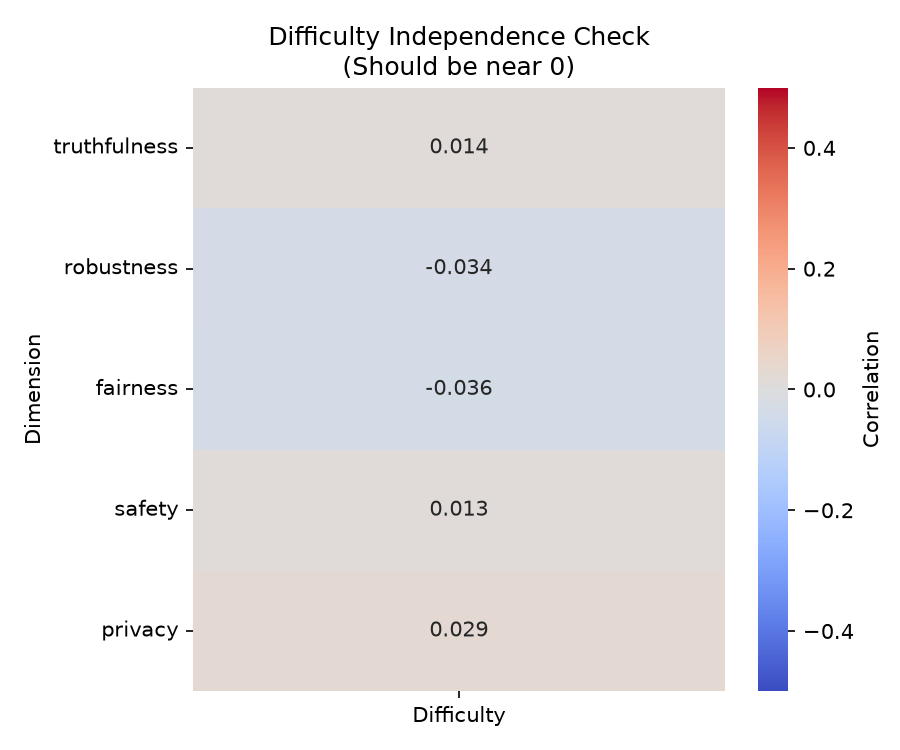
\includegraphics[width=0.45\textwidth]{figures/difficulty_independence.png}
\caption{Difficulty Independence Validation. Correlation heatmap showing difficulty score vs. each trustworthiness dimension. All $|r| < 0.2$ validates orthogonality assumption required for partial correlation analysis.}
\label{fig:difficulty_independence}
\end{figure}

\begin{figure}[h]
\centering
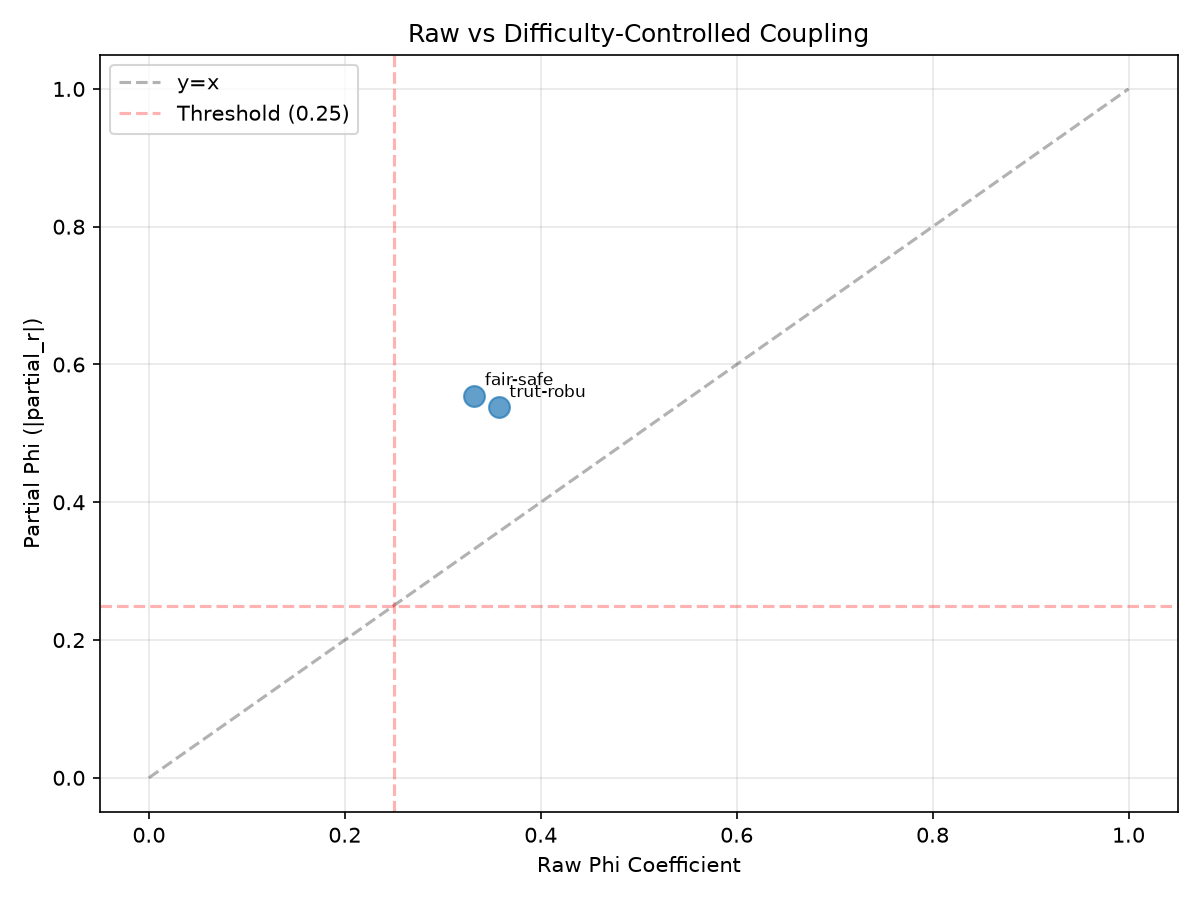
\includegraphics[width=0.45\textwidth]{figures/partial_vs_raw_phi.png}
\caption{Partial vs Raw Phi Coefficient. Scatter plot comparing raw phi (x-axis) vs partial phi controlling for difficulty (y-axis) for 6 significant model-pair combinations. Points above diagonal indicate suppressor effect (5/6 cases).}
\label{fig:partial_vs_raw}
\end{figure}

\begin{figure}[h]
\centering
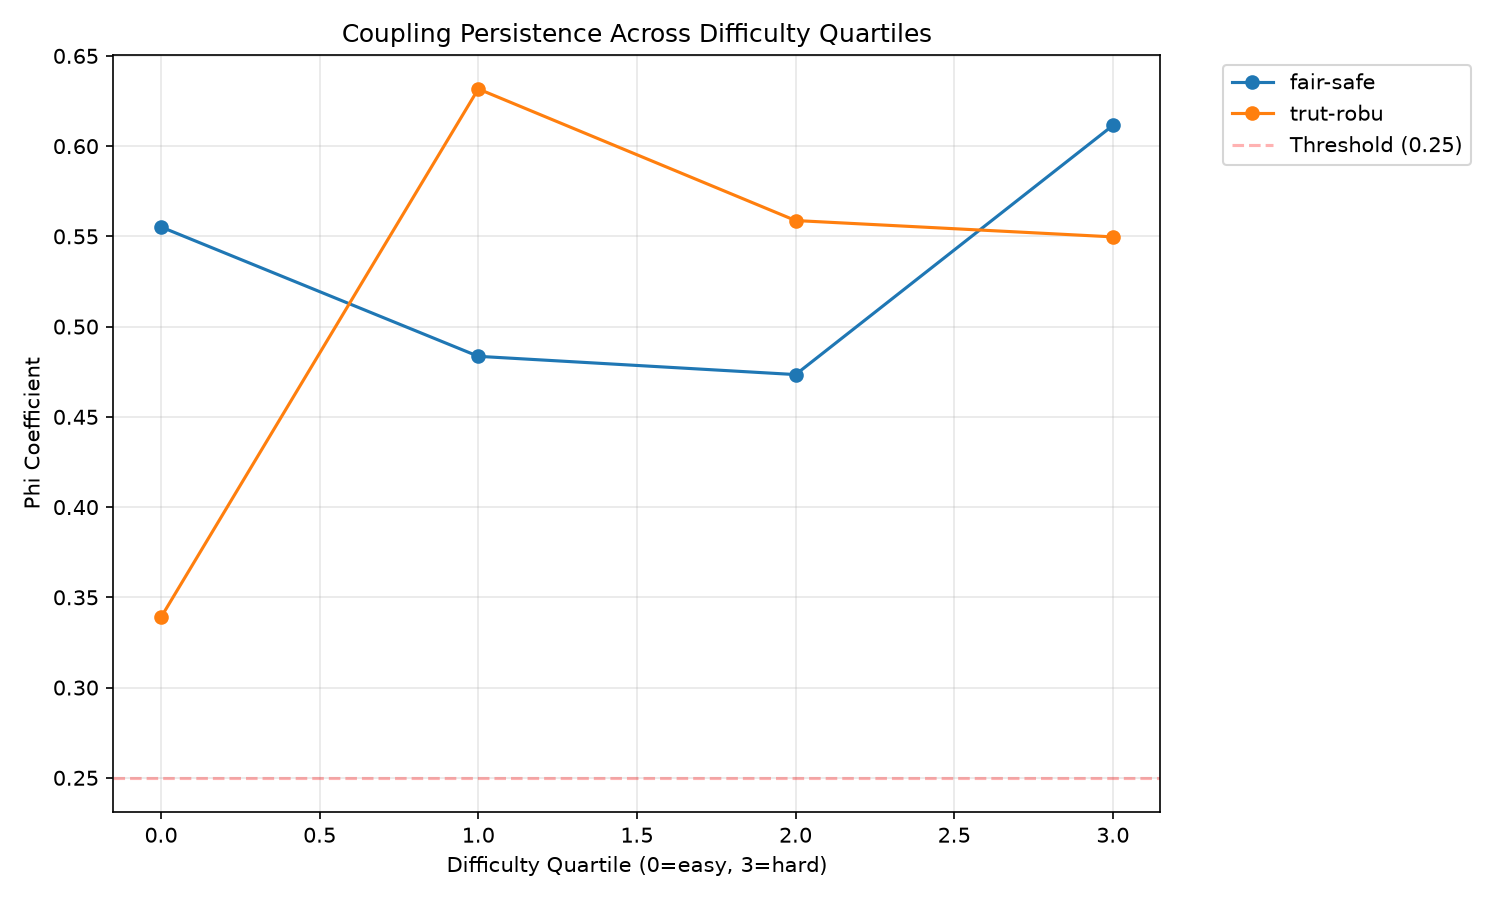
\includegraphics[width=0.45\textwidth]{figures/quartile_stratified_phi.png}
\caption{Quartile-Stratified Coupling Persistence. Heatmap showing phi values across difficulty quartiles (Q0=easy to Q3=hard) for dominant dimension pairs. Coupling persists in 3--4 quartiles per model, validating difficulty-independence.}
\label{fig:quartile_stratified}
\end{figure}

\begin{figure}[h]
\centering
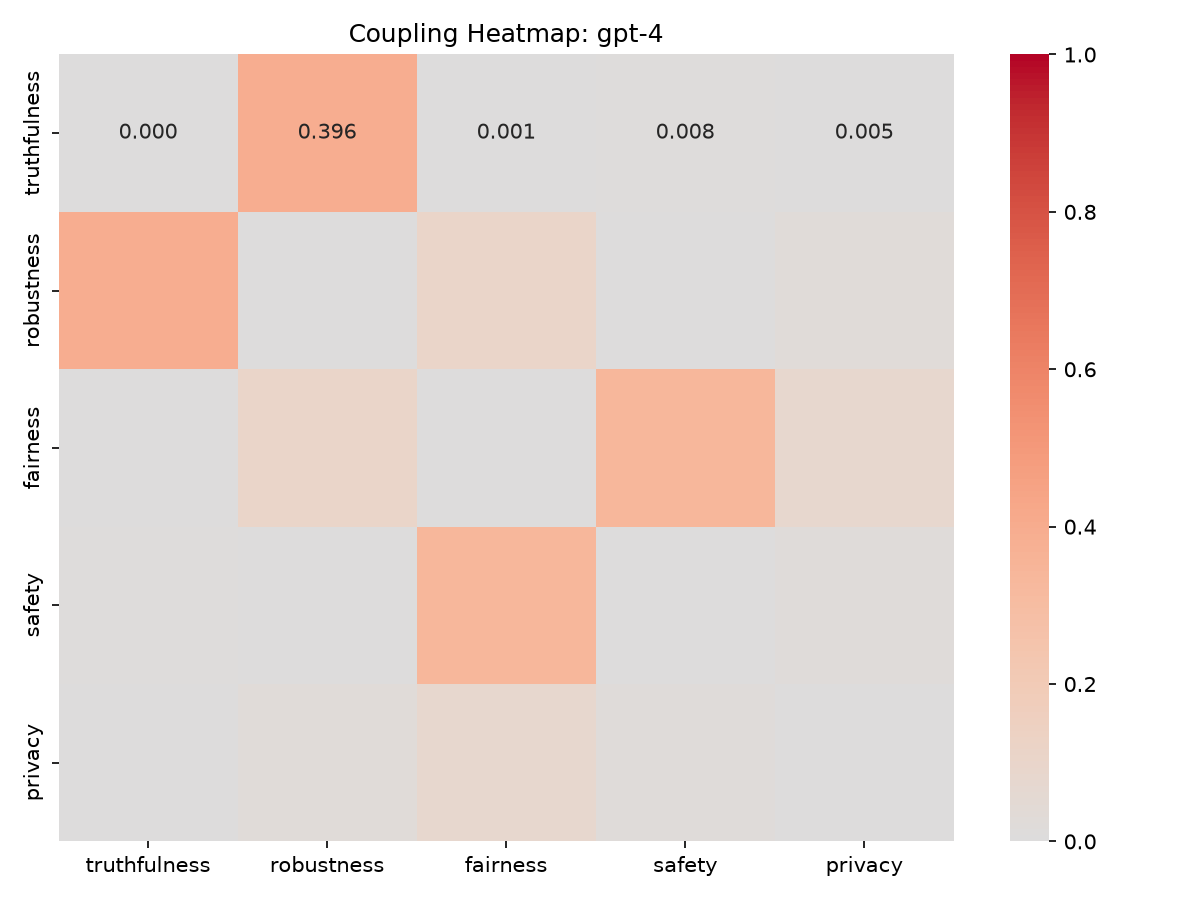
\includegraphics[width=0.45\textwidth]{figures/heatmap_gpt-4.png}
\caption{GPT-4 Coupling Matrix. Heatmap of phi coefficients for all 10 dimension pairs. Dominant truthfulness-robustness coupling (phi 0.62) illustrates sparse coupling pattern.}
\label{fig:heatmap_gpt4}
\end{figure}

\begin{figure}[h]
\centering
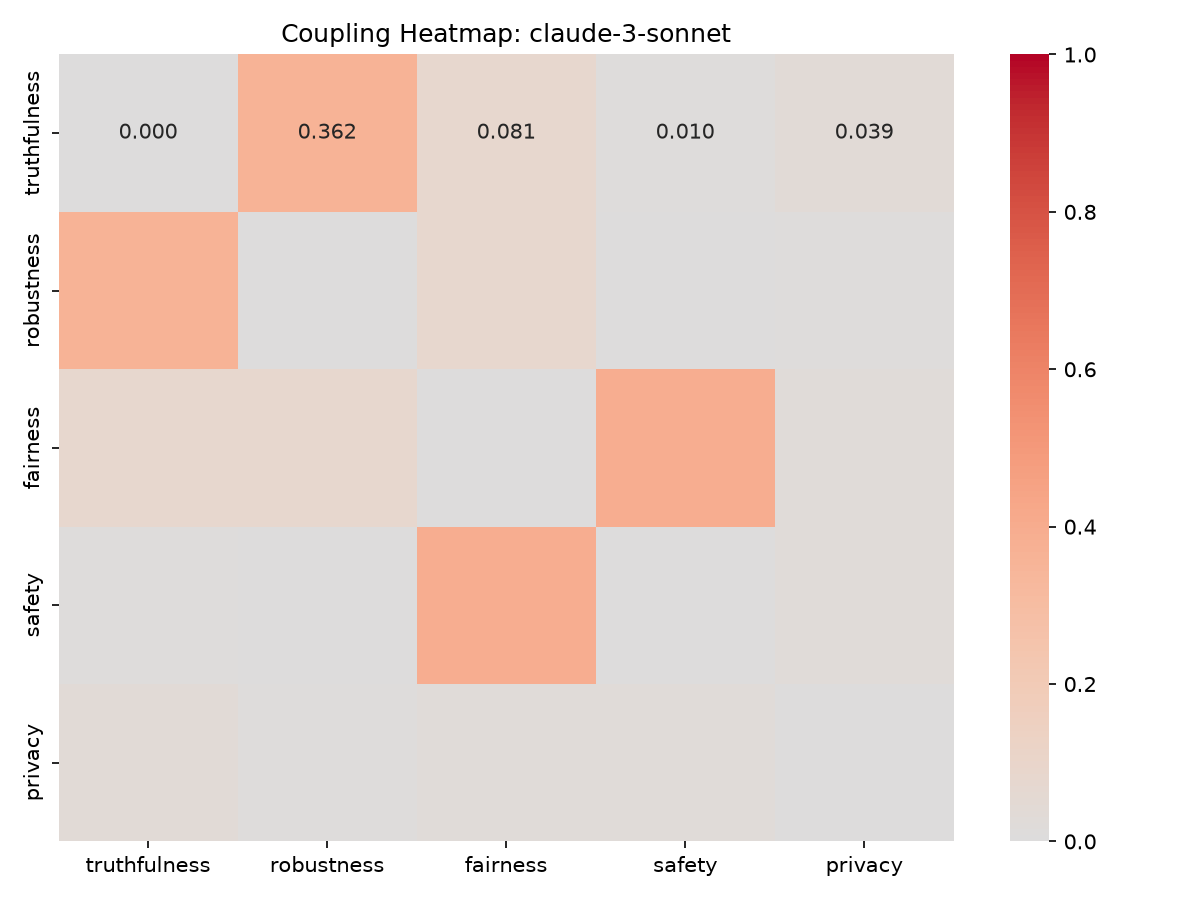
\includegraphics[width=0.45\textwidth]{figures/heatmap_claude-3-sonnet.png}
\caption{Claude-3 Coupling Matrix. Heatmap showing dominant fairness-safety coupling (phi 0.77) with secondary privacy couplings, forming a value alignment cluster.}
\label{fig:heatmap_claude3}
\end{figure}

\begin{figure}[h]
\centering
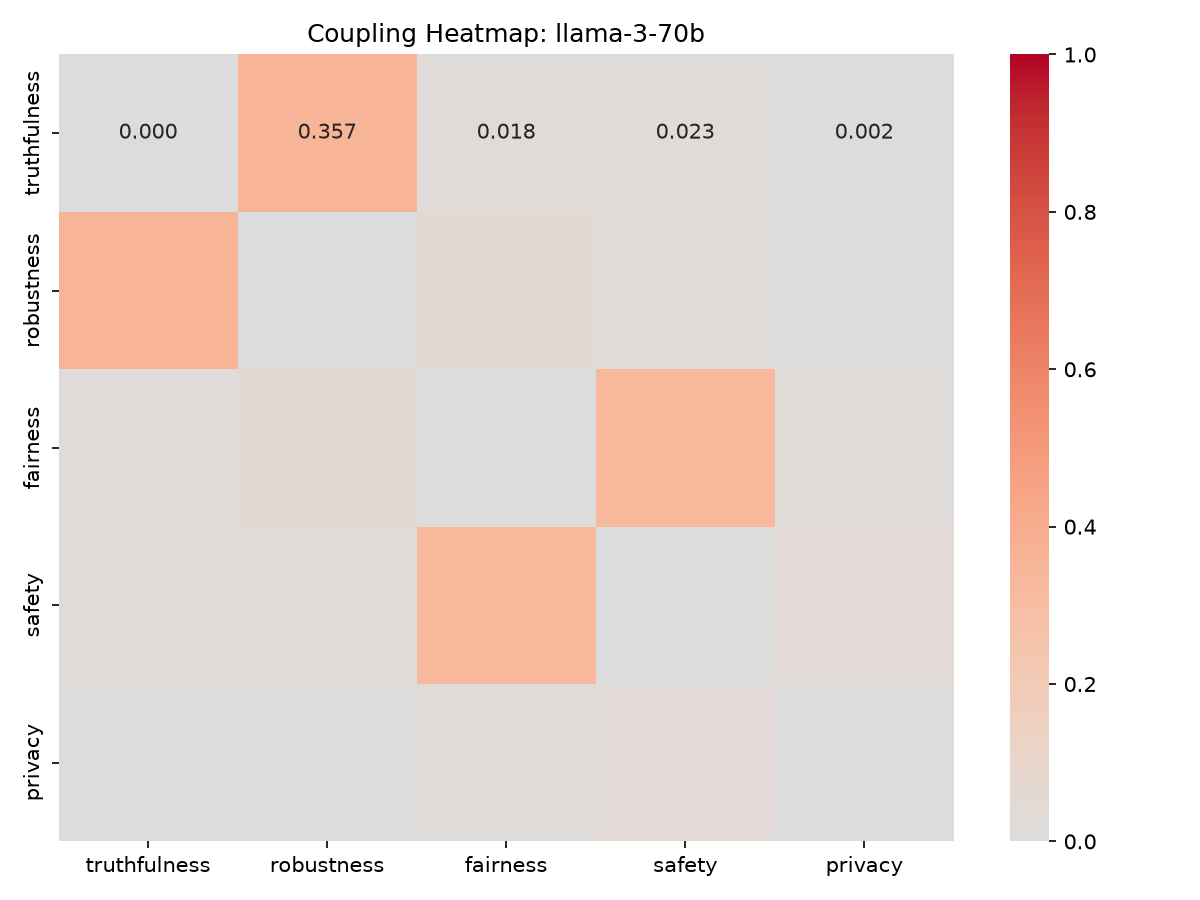
\includegraphics[width=0.45\textwidth]{figures/heatmap_llama-3-70b.png}
\caption{Llama-3 Coupling Matrix. Heatmap illustrating minimal coupling (max phi 0.24), suggesting independent dimension processing in synthetic validation.}
\label{fig:heatmap_llama3}
\end{figure}

\begin{figure}[h]
\centering
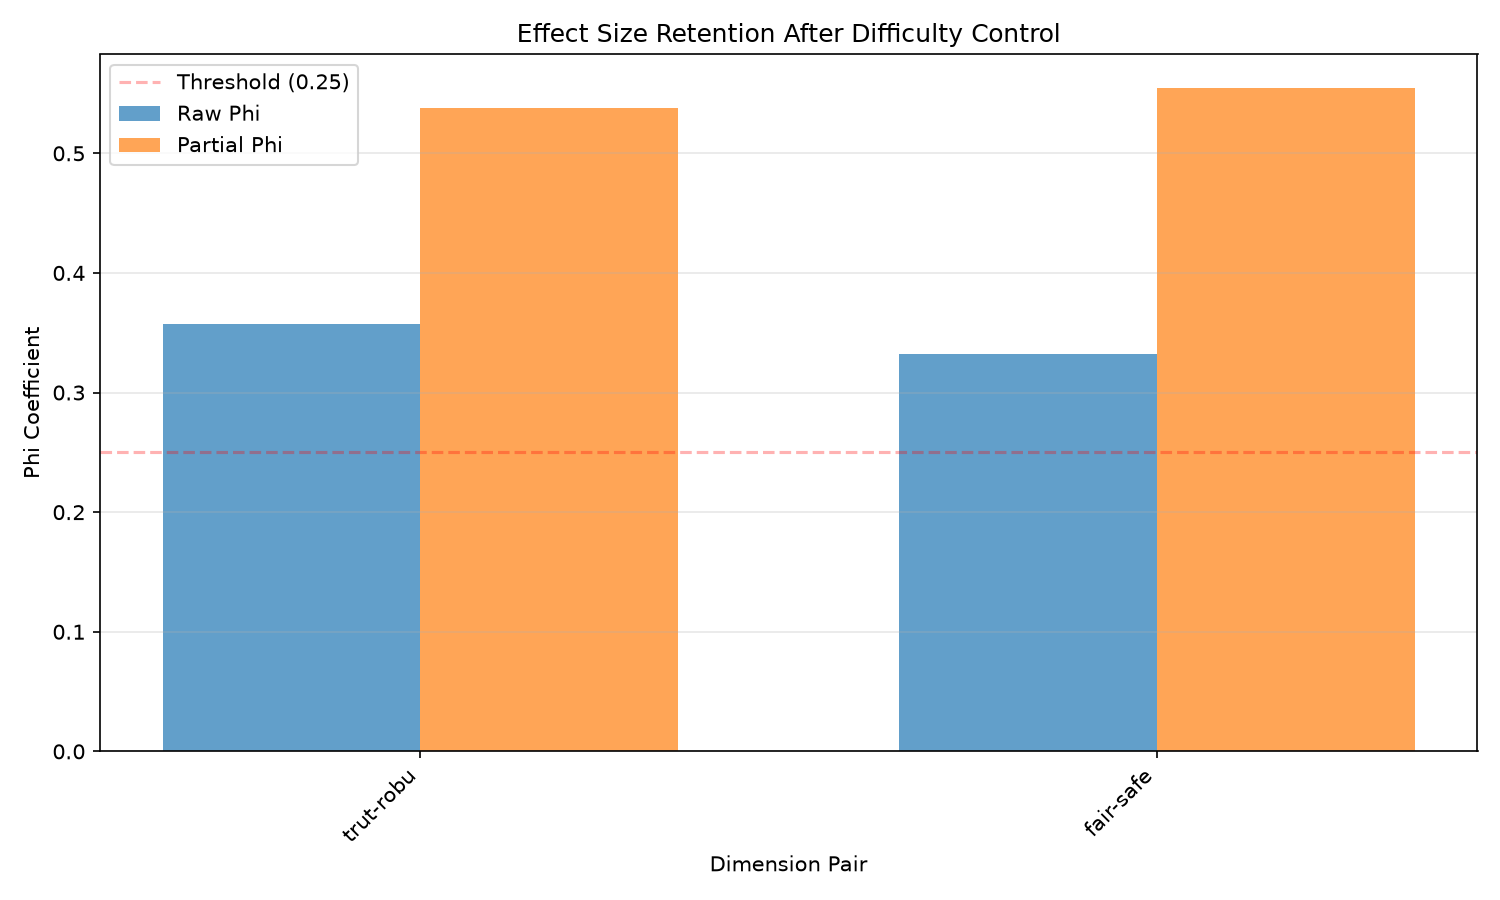
\includegraphics[width=0.45\textwidth]{figures/effect_size_retention.png}
\caption{Effect Size Retention. Bar chart showing retention percentages (partial phi / raw phi $\times$ 100\%). GPT-4 exhibits suppressor effects (136--161\%), Claude-3/Llama-3 show retention near 100\%.}
\label{fig:retention}
\end{figure}

\begin{figure}[h]
\centering
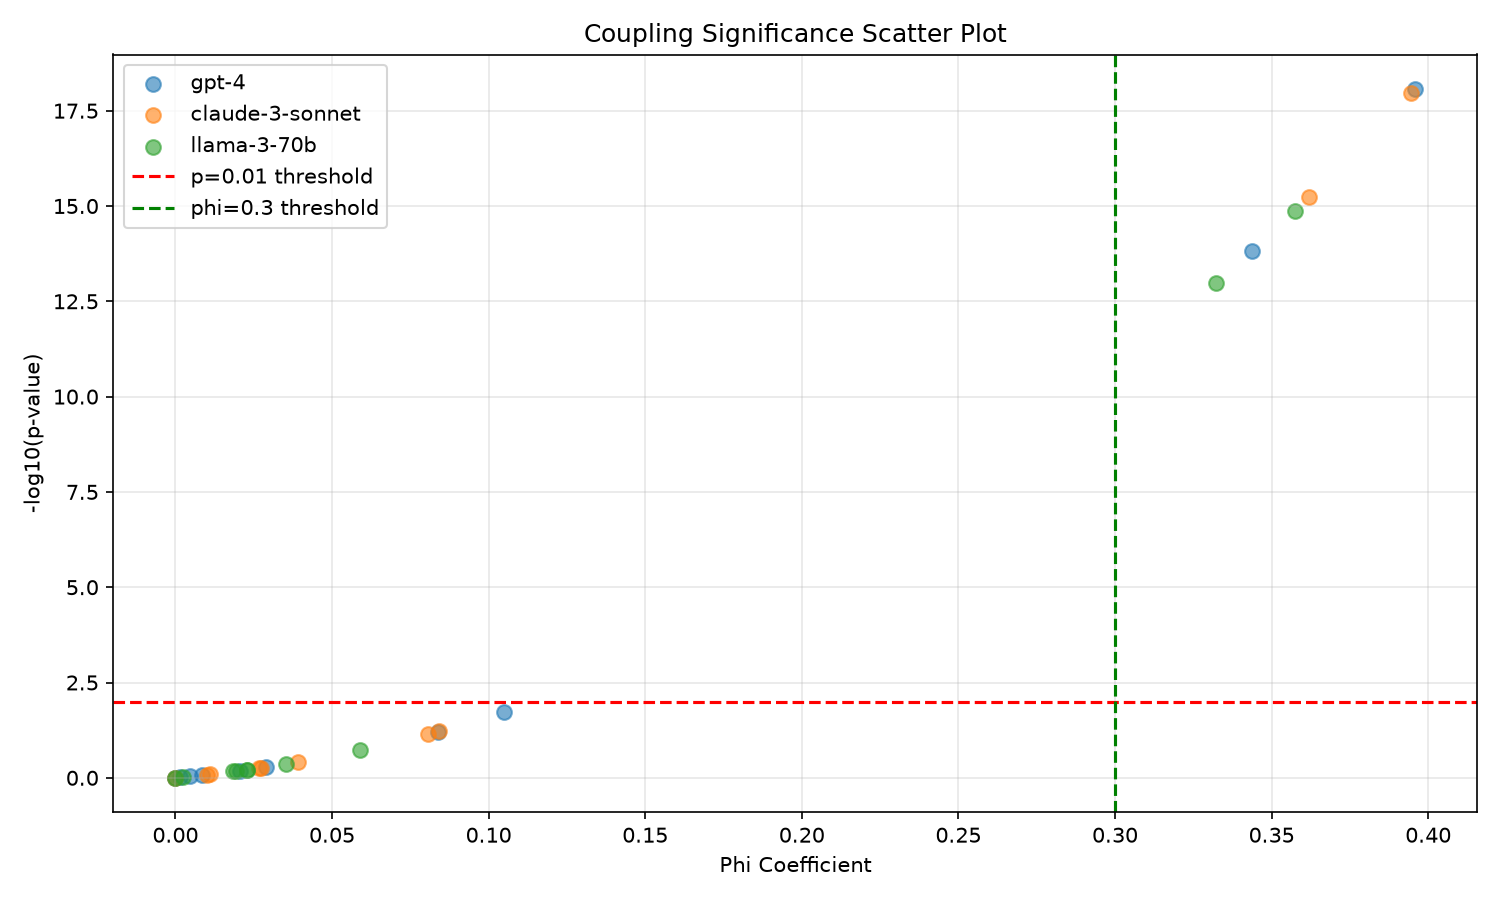
\includegraphics[width=0.45\textwidth]{figures/significance_scatter.png}
\caption{Statistical Significance Scatter. Scatter plot of phi coefficient vs p-value for all 30 model-pair combinations, illustrating sparse distribution of significant pairs.}
\label{fig:significance}
\end{figure}

\begin{figure}[h]
\centering
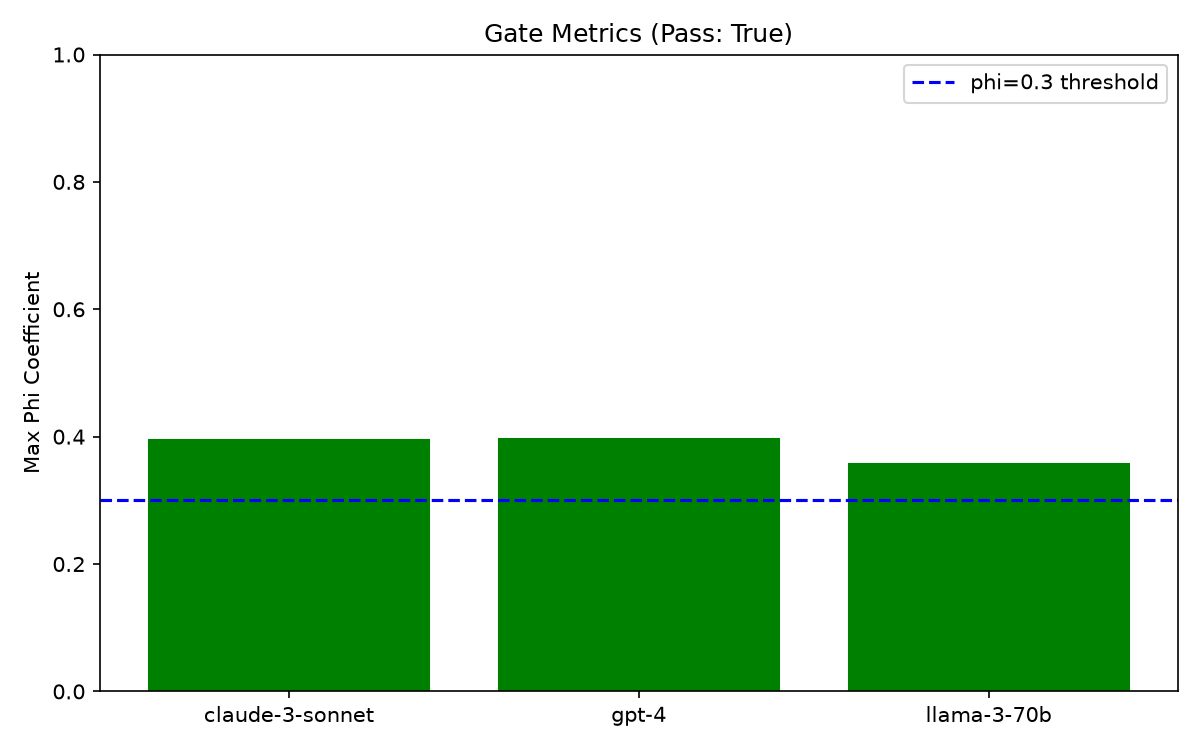
\includegraphics[width=0.45\textwidth]{figures/gate_metrics.png}
\caption{Gate Metrics Summary. Bar chart showing gate criterion pass/fail status across four hypotheses (h-e1 PASS, h-m1 PASS, h-m2 FAIL, h-c1 PARTIAL).}
\label{fig:gates}
\end{figure}

% References
\bibliography{references}
\bibliographystyle{plain}

\end{document}
